\documentclass[conference]{IEEEtran}
\usepackage{cite}
\usepackage{amsmath,amssymb,amsfonts}
\usepackage{graphicx}
\usepackage{float}
\usepackage{textcomp}
\usepackage{booktabs}
\usepackage{siunitx}
\usepackage{multirow}
\usepackage{url}
\def\UrlBreaks{\do\/\do-}
\usepackage[hidelinks]{hyperref}
\graphicspath{{source/extracted_images/}}

\begin{document}

\title{Design, Modeling, Optimization, and Evaluation of a Soil Electrical Conductivity Sensor for Precision Agriculture}

\author{
\IEEEauthorblockN{Andrew Khalil}
\IEEEauthorblockA{\textit{Dept. of Mechatronics Engineering} \\
\textit{German University in Cairo (GUC)}\\
Cairo, Egypt}
\and
\IEEEauthorblockN{Daniel George}
\IEEEauthorblockA{\textit{Dept. of Mechatronics Engineering} \\
\textit{German University in Cairo (GUC)}\\
Cairo, Egypt}
\and
\IEEEauthorblockN{David Louis}
\IEEEauthorblockA{\textit{Dept. of Mechatronics Engineering} \\
\textit{German University in Cairo (GUC)}\\
Cairo, Egypt}
\and
\IEEEauthorblockN{Samir Sameh}
\IEEEauthorblockA{\textit{Dept. of Mechatronics Engineering} \\
\textit{German University in Cairo (GUC)}\\
Cairo, Egypt}
\and
\IEEEauthorblockN{Youssef Youssry}
\IEEEauthorblockA{\textit{Dept. of Mechatronics Engineering} \\
\textit{German University in Cairo (GUC)}\\
Cairo, Egypt}
}

\maketitle

\begin{abstract}
This paper presents the complete design, mathematical modeling, performance optimization, signal processing, and commercial benchmarking of a two-electrode soil electrical conductivity (EC) sensor for precision agriculture applications. The sensor is modeled as a second-order RLC circuit using the Lagrangian energy approach, yielding the transfer function $H(s) = C_{dl}s / (L_{coil}C_{dl}s^2 + R_{soil}C_{dl}s + 1)$ with baseline parameters $L_{coil}=3\,\mu$H, $C_{dl}=10\,\mu$F, and $R_{soil}=5$\,\si{\ohm} to $200$\,k\si{\ohm}. Baseline characterization reveals a natural frequency of $f_n \approx 29.06$\,kHz, a non-linearity error of 76.8\% FSO, and a damping ratio varying from $\zeta \approx 45$ (saline) to $\zeta \approx 136{,}931$ (fresh water). To address sluggish response ($\tau = 1.5$\,s) and poor fresh-water sensitivity ($I_{peak} = 6.67\,\mu$A), a geometric optimization strategy reduces the cell constant from $K_{cell} = 1.0$ to $0.1\,\text{cm}^{-1}$, achieving a 10$\times$ sensitivity gain, a 5$\times$ RC time-constant improvement ($\tau = 0.3$\,s), and practical current settling in less than 100\,ms. A dual-window moving average compensation algorithm is implemented to mitigate 30\,dB SNR noise and 8\% amplitude drift. Finally, a weighted decision matrix compares the optimized design against three commercial sensors (Atlas Scientific K\,1.0, Vernier CON-BTA, METER 5TE), with the Atlas Scientific K\,1.0 achieving the highest score of 9.00/10 for wide-range agricultural monitoring.
\end{abstract}

\begin{IEEEkeywords}
Soil electrical conductivity, salinity sensor, RLC circuit modeling, Lagrangian dynamics, geometric optimization, signal processing, precision agriculture.
\end{IEEEkeywords}

\section{Introduction}
Soil electrical conductivity (EC) measurement is fundamental to precision agriculture, enabling real-time assessment of soil salinity for irrigation management, fertilizer optimization, and long-term soil health monitoring~\cite{atlas2023}. Excessive salinity inhibits plant water uptake, reduces crop yields, and can cause permanent soil degradation, particularly in arid and semi-arid regions~\cite{vernier2025,rhoades1999,ayers1985}.

Two-electrode conductivity probes offer a cost-effective and non-destructive approach to EC measurement~\cite{corwin2005,fraden2016}. The sensing principle relies on ionic conduction: dissolved salts in the soil moisture facilitate current flow between two inert electrodes separated by a fixed distance. The soil acts as a variable resistor $R_{soil}$, inversely proportional to EC according to the geometric cell constant $K_{cell}$:
\begin{equation}
R_{soil} = \frac{K_{cell}}{EC}, \quad K_{cell} \approx \frac{d}{A}
\label{eq:rsoil}
\end{equation}
where $d$ is the inter-electrode spacing and $A$ is the electrode surface area. To prevent electrode polarization and the formation of an insulating double-layer, AC excitation at $f_{ex} = 1$\,kHz is employed.

This paper presents a comprehensive study spanning four phases: (1)~Lagrangian-based mathematical modeling and baseline characterization; (2)~geometric optimization for improved sensitivity and dynamic response; (3)~noise and drift compensation via digital signal processing; and (4)~evaluation against commercial sensor datasheets using a weighted decision matrix. The contributions include the derivation of a complete second-order transfer function from energy principles, quantitative identification of performance limitations, a physics-informed optimization strategy yielding 10$\times$ sensitivity gain and $>$60$\times$ faster settling, and a systematic commercial benchmarking framework.

\section{Mathematical Modeling}
\subsection{Lagrangian Derivation of the RLC Model}
The sensor system is modeled as a series RLC circuit comprising the lead inductance $L_{coil}$, the variable soil resistance $R_{soil}$, and the probe double-layer capacitance $C_{dl}$. Using the Lagrangian energy approach with charge $q(t)$ as the generalized coordinate, the kinetic co-energy, potential energy, and Rayleigh dissipation function are:
\begin{equation}
T^* = \frac{1}{2}L_{coil}\dot{q}^2, \quad V = \frac{q^2}{2C_{dl}}, \quad \mathcal{D} = \frac{1}{2}R_{soil}\dot{q}^2
\end{equation}
Applying the Euler--Lagrange equation with dissipation:
\begin{equation}
\frac{d}{dt}\frac{\partial T^*}{\partial \dot{q}} - \frac{\partial T^*}{\partial q} + \frac{\partial V}{\partial q} + \frac{\partial \mathcal{D}}{\partial \dot{q}} = V_{in}(t)
\end{equation}
yields the governing differential equation:
\begin{equation}
L_{coil}\ddot{q}(t) + R_{soil}\dot{q}(t) + \frac{1}{C_{dl}}q(t) = V_{in}(t)
\label{eq:ode}
\end{equation}
where $V_{in}(t) = V_{peak}\sin(2\pi f_{ex}t)$ is the AC excitation.

\subsection{Transfer Function and State-Space Formulation}
Since the output current is $I(t) = \dot{q}(t)$, Laplace transformation of~(\ref{eq:ode}) yields the admittance transfer function~\cite{ogata2010}:
\begin{equation}
H(s) = \frac{I(s)}{V_{in}(s)} = \frac{C_{dl}s}{L_{coil}C_{dl}s^2 + R_{soil}C_{dl}s + 1}
\label{eq:tf}
\end{equation}
The state-space formulation with state vector $\mathbf{x} = [q,\; \dot{q}]^T$ is:
\begin{equation}
\dot{\mathbf{x}} = \begin{bmatrix} 0 & 1 \\ -\frac{1}{L_{coil}C_{dl}} & -\frac{R_{soil}}{L_{coil}} \end{bmatrix}\mathbf{x} + \begin{bmatrix} 0 \\ \frac{1}{L_{coil}} \end{bmatrix}V_{in}
\end{equation}
with output $I = [0\;\; 1]\,\mathbf{x}$.

\subsection{Baseline Sensor Parameters}
Table~\ref{tab:baseline_params} summarizes the baseline parameters selected based on the Atlas Scientific K\,1.0 probe geometry~\cite{atlas2023}.

\begin{table}[H]
\centering
\caption{Baseline Sensor Parameters}
\label{tab:baseline_params}
\begin{tabular}{lll}
\toprule
\textbf{Parameter} & \textbf{Symbol} & \textbf{Value} \\
\midrule
Lead Inductance & $L_{coil}$ & $3\,\mu$H \\
Double-Layer Capacitance & $C_{dl}$ & $10\,\mu$F \\
Cell Constant & $K_{cell}$ & $1.0\,\text{cm}^{-1}$ \\
Excitation Frequency & $f_{ex}$ & 1\,kHz \\
Excitation Voltage & $V_{peak}$ & 1\,V \\
Soil Resistance Range & $R_{soil}$ & 5\,\si{\ohm}--200\,k\si{\ohm} \\
\bottomrule
\end{tabular}
\end{table}

\section{Baseline Characterization}
\subsection{Dynamic Response}
MATLAB simulation of the baseline system at $R_{soil} = 10$\,k\si{\ohm} confirms stable sinusoidal current output at 1\,kHz, as shown in Fig.~\ref{fig:ms1_dynamic}. The system exhibits no overshoot or ringing due to heavy overdamping.

\begin{figure}[H]
\centering
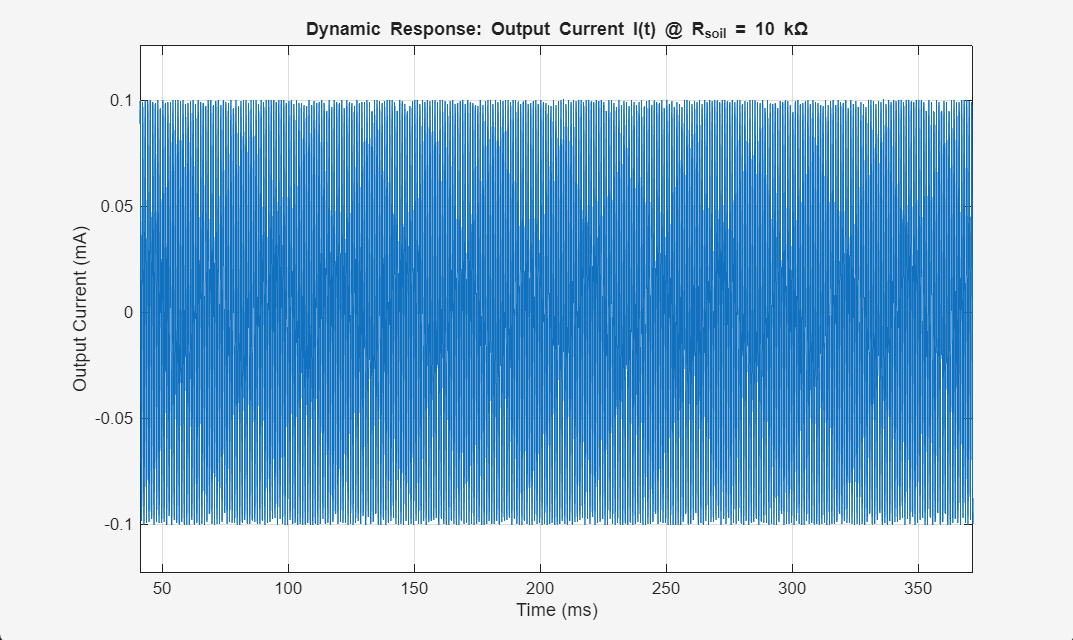
\includegraphics[width=\columnwidth]{page4_img1.jpeg}
\caption{Baseline dynamic response: output current $I(t)$ at $R_{soil} = 10$\,k\si{\ohm} showing stable sinusoidal output at 1\,kHz excitation.}
\label{fig:ms1_dynamic}
\end{figure}

The natural frequency and damping ratio are:
\begin{equation}
f_n = \frac{1}{2\pi\sqrt{L_{coil}C_{dl}}} \approx 29.06\;\text{kHz}
\end{equation}
\begin{equation}
\zeta = \frac{R_{soil}}{2}\sqrt{\frac{C_{dl}}{L_{coil}}}
\end{equation}
Since $f_{ex} = 1$\,kHz is well below $f_n$, the sensor operates in the flat passband of the frequency response. However, the damping ratio varies dramatically with soil conditions: $\zeta \approx 45$ for salty water ($R_{soil} = 50$\,\si{\ohm}) to $\zeta \approx 136{,}931$ for fresh water ($R_{soil} = 150$\,k\si{\ohm}).

\subsection{Static Response and Non-Linearity}
The static calibration curve (Fig.~\ref{fig:ms1_static}) reveals a strong inverse relationship $I \propto 1/R_{soil}$, yielding a non-linearity error of 76.8\% FSO when fitted against a best-fit straight line (Fig.~\ref{fig:ms1_linearity}). The sensitivity is highly non-uniform: adequate in saline conditions but dropping to $I_{peak} \approx 6.67\,\mu$A in fresh water ($R_{soil} = 150$\,k\si{\ohm}), rendering the output indistinguishable from circuit noise.

\begin{figure}[H]
\centering
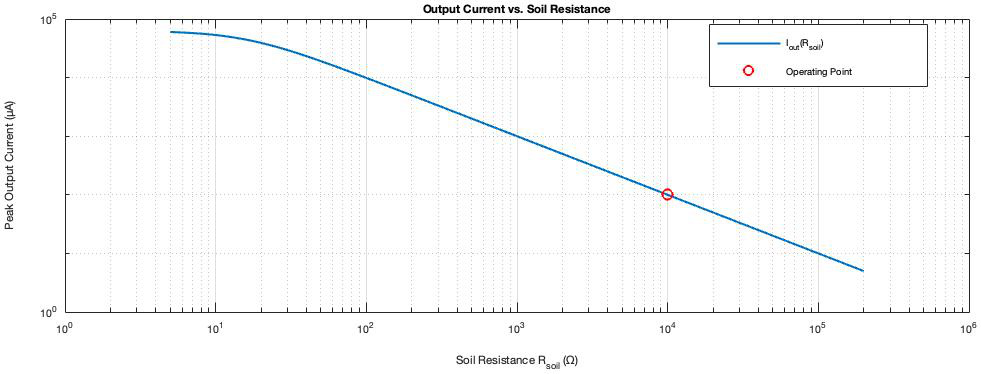
\includegraphics[width=\columnwidth]{page4_img2.jpeg}
\caption{Baseline static response: peak output current vs.\ soil resistance on a log-log scale, showing the inverse $I \propto 1/R_{soil}$ relationship.}
\label{fig:ms1_static}
\end{figure}

\begin{figure}[H]
\centering
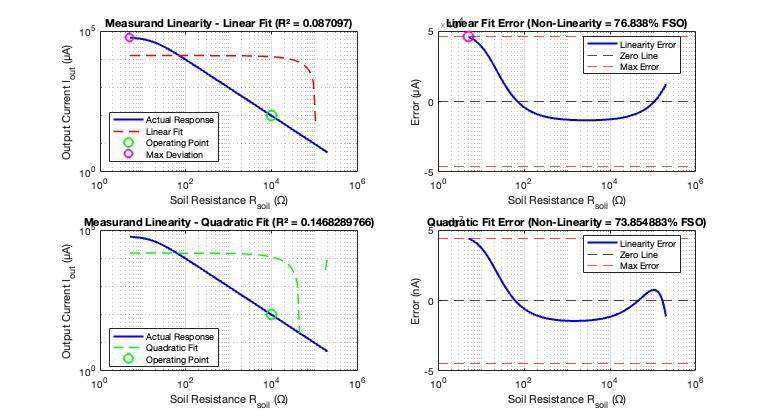
\includegraphics[width=\columnwidth]{page5_img1.jpeg}
\caption{Linearity analysis: linear and quadratic fits to the static response with non-linearity errors of 76.8\% and 73.9\% FSO, respectively.}
\label{fig:ms1_linearity}
\end{figure}

\subsection{Frequency Response}
Fig.~\ref{fig:ms1_bode} presents the Bode plot at $R_{soil} = 10$\,k\si{\ohm}. The magnitude is flat from approximately 10\,Hz to the natural frequency at 29\,kHz, with the $-3$\,dB bandwidth exceeding 1\,MHz. The operating frequency (1\,kHz) falls well within the passband, confirming stable AC operation without resonance effects.

\begin{figure}[H]
\centering
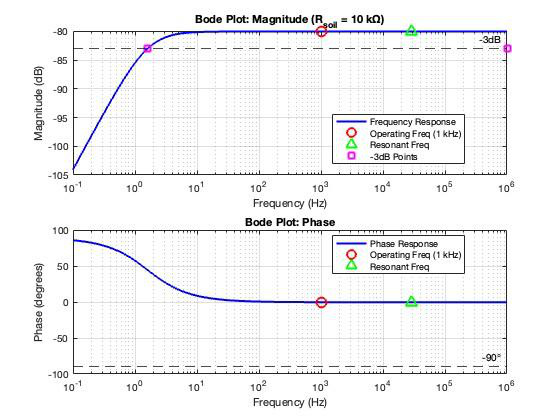
\includegraphics[width=0.85\columnwidth]{page5_img2.jpeg}
\caption{Baseline Bode plot at $R_{soil} = 10$\,k\si{\ohm}: magnitude and phase vs.\ frequency, showing flat response at 1\,kHz and natural resonance at $\approx$29\,kHz.}
\label{fig:ms1_bode}
\end{figure}

Table~\ref{tab:baseline_perf} summarizes the baseline performance metrics.

\begin{table}[H]
\centering
\caption{Baseline Performance Metrics}
\label{tab:baseline_perf}
\begin{tabular}{lll}
\toprule
\textbf{Metric} & \textbf{Value} & \textbf{Condition} \\
\midrule
Natural Frequency & 29.06\,kHz & Theoretical \\
Non-Linearity & 76.8\% FSO & Inverse $I$--$R$ \\
Min Output Current & $6.67\,\mu$A & Fresh Water (150\,k\si{\ohm}) \\
Max Damping Ratio & $\zeta \approx 136{,}931$ & Fresh Water \\
Time Constant & 1.5\,s & $\tau = R_{soil} \cdot C_{dl}$ \\
Settling Time & $\approx$6\,s & $t_s \approx 4\tau$ \\
\bottomrule
\end{tabular}
\end{table}

\section{Geometric Optimization}
\subsection{Identified Limitations}
The baseline characterization reveals three critical limitations in fresh water conditions: (1)~severe non-linearity (76.8\% FSO) due to the inherent $I \propto 1/R$ relationship; (2)~poor sensitivity with output current as low as $6.67\,\mu$A, yielding inadequate SNR; and (3)~sluggish dynamic response with $\tau = 1.5$\,s and settling time $\approx$6\,s, unsuitable for real-time irrigation control.

\subsection{Optimization Strategy}
The proposed improvement reduces the cell constant from $K_{cell} = 1.0$ to $0.1\,\text{cm}^{-1}$ by decreasing the inter-electrode spacing $d$ and increasing the electrode surface area $A$. This geometric modification has three effects:

\textbf{Sensitivity:} Since $R_{soil} = K_{cell}/EC$, reducing $K_{cell}$ by 10$\times$ reduces soil resistance by 10$\times$ for constant EC. Because $I \approx V/R_{soil}$, the output current increases by 10$\times$.

\textbf{Response Time:} The time constant $\tau = R_{soil} \cdot C_{dl}$ decreases because $R_{soil}$ drops. Even though the larger electrode area approximately doubles $C_{dl}$ (from 10 to 20\,$\mu$F), the net effect is a 5$\times$ speed improvement.

\textbf{Polarization:} Increasing electrode area $A$ reduces current density $J = I/A$, thereby mitigating electrode polarization impedance.

\subsection{Updated Parameters and Theoretical Predictions}
The optimized parameters are:
\begin{align}
R_{soil,new} &= R_{soil,base} \times \frac{K_{new}}{K_{old}} = 150\,\text{k\si{\ohm}} \times 0.1 = 15\,\text{k\si{\ohm}} \label{eq:rnew}\\
C_{dl,new} &\approx 2 \times C_{dl,base} = 20\,\mu\text{F} \label{eq:cnew}\\
\tau_{new} &= R_{new} \cdot C_{new} = 15\,\text{k\si{\ohm}} \times 20\,\mu\text{F} = 0.3\,\text{s} \label{eq:taunew}
\end{align}
The improvement factor is $\tau_{base}/\tau_{new} = 1.5/0.3 = 5$.

\subsection{Simulation Validation}
Fig.~\ref{fig:ms2_dynamic} shows the optimized dynamic response at $R_{soil} = 15$\,k\si{\ohm}. The sensor achieves AC steady state within $t_s < 0.2$\,ms (well below one period of 1\,kHz excitation) with a stable peak current of $66.67\,\mu$A. In step-current terms, the fast inductive rise time constant is $\tau_L = L_{coil}/R_{soil} = 0.2$\,ns, while the slow double-layer RC charging time constant drops $5\times$ ($\tau_{RC} = 1.5\,\text{s} \rightarrow 0.3\,\text{s}$, 2\% decay time $5.87\,\text{s} \rightarrow 1.17\,\text{s}$). At $f_{ex} = 1$\,kHz, capacitive reactance $|Z_C| = 1/(2\pi f_{ex} C_{dl}) \approx 7.96$\,\si{\ohm} is negligible compared to $R_{soil} = 15$\,k\si{\ohm}, so the resistive response $I(t) \approx V_{peak}\sin(2\pi f_{ex}t)/R_{soil}$ dominates and AC settling occurs in under one cycle.

\begin{figure}[H]
\centering
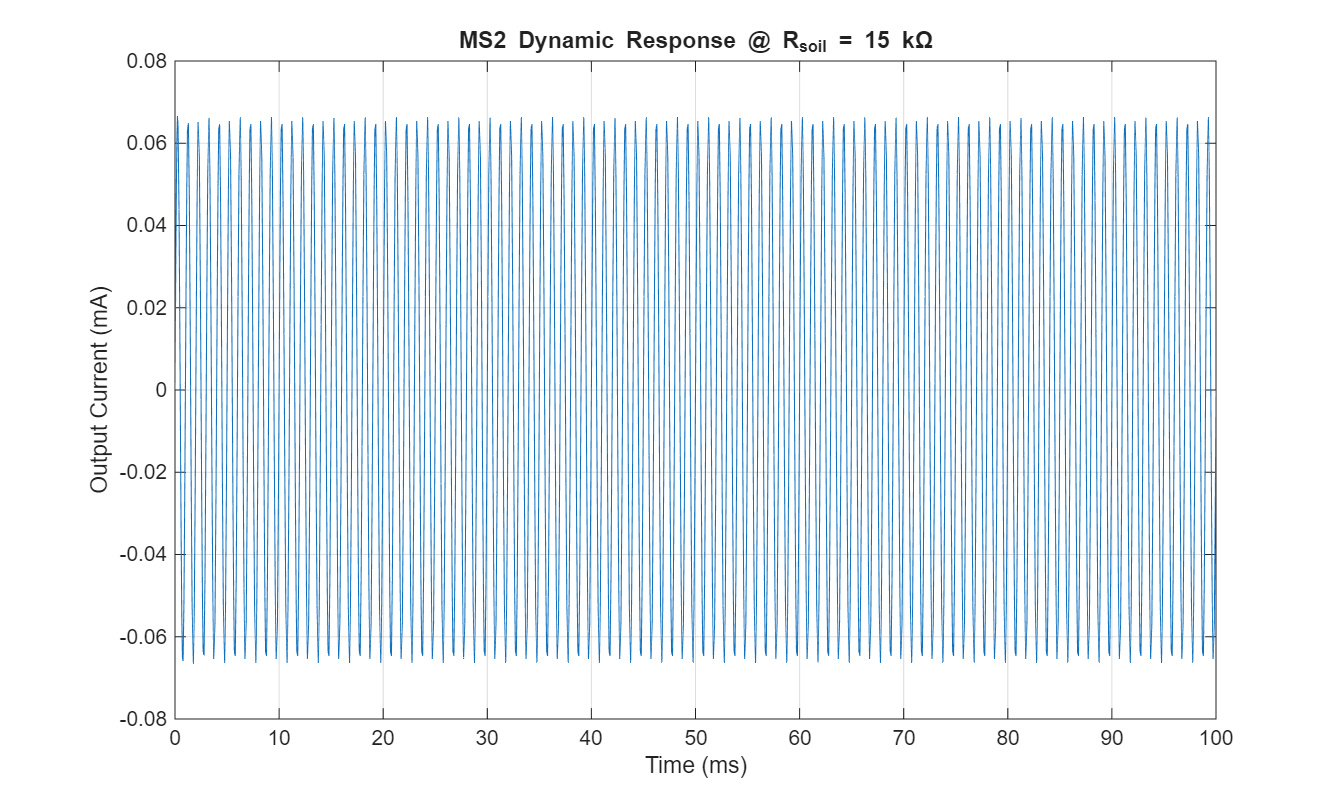
\includegraphics[width=\columnwidth]{page13_img1.jpeg}
\caption{Optimized dynamic response at $R_{soil} = 15$\,k\si{\ohm}: fast settling ($<$0.2\,ms) and stable 1\,kHz sinusoidal output with peak amplitude $\approx$67\,$\mu$A.}
\label{fig:ms2_dynamic}
\end{figure}

The optimized static calibration (Fig.~\ref{fig:ms2_static}) confirms a wide dynamic range spanning more than four decades of resistance (5\,\si{\ohm} to 200\,k\si{\ohm}), with the fresh-water current elevated to $66.7\,\mu$A---a 10$\times$ improvement providing adequate SNR for practical measurement.

\begin{figure}[H]
\centering
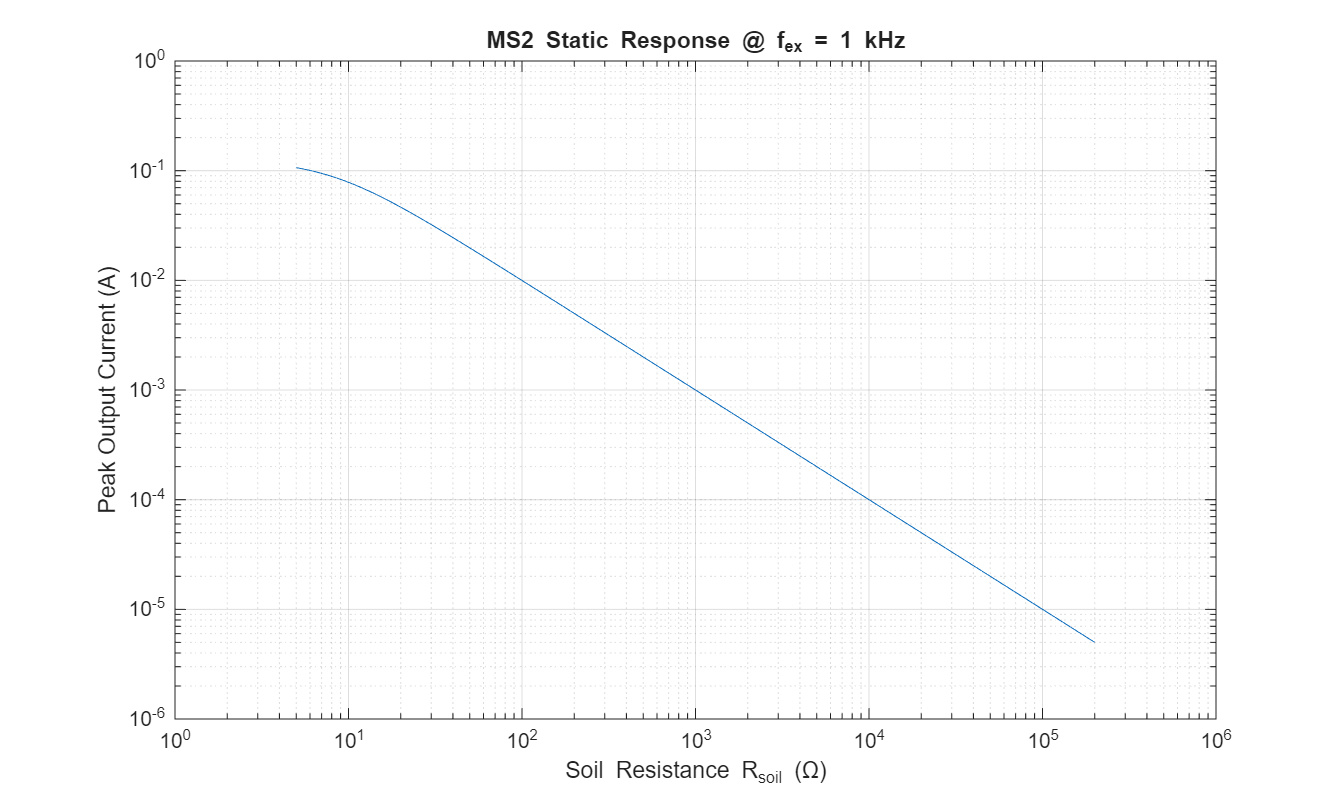
\includegraphics[width=\columnwidth]{page13_img2.jpeg}
\caption{Optimized static calibration: peak output current vs.\ soil resistance over four decades, showing 10$\times$ improved sensitivity at the fresh-water operating point.}
\label{fig:ms2_static}
\end{figure}

Table~\ref{tab:optimization} compares baseline and optimized performance.

\begin{table}[H]
\centering
\caption{Performance Comparison: Baseline vs.\ Optimized Design}
\label{tab:optimization}
\begin{tabular}{llll}
\toprule
\textbf{Metric} & \textbf{Baseline} & \textbf{Optimized} & \textbf{Factor} \\
\midrule
$K_{cell}$ [cm$^{-1}$] & 1.0 & 0.1 & 10$\times$ $\downarrow$ \\
$C_{dl}$ [$\mu$F] & 10 & 20 & 2$\times$ $\uparrow$ \\
$R_{soil}$ [k\si{\ohm}] & 150 & 15 & 10$\times$ $\downarrow$ \\
$\tau_{RC}$ [s] & 1.5 & 0.3 & 5$\times$ faster \\
Settling Time & $\approx$6\,s & $<$100\,ms & $>$60$\times$ faster \\
$I_{peak}$ (fresh) [$\mu$A] & 6.67 & 66.7 & 10$\times$ $\uparrow$ \\
$f_n$ [kHz] & 29.06 & 20.5 & -- \\
Bandwidth & $>$1\,MHz & $>$2\,MHz & $\sim$2$\times$ \\
\bottomrule
\end{tabular}
\end{table}

\section{Noise and Drift Compensation}
\subsection{Impairment Model}
Real-world deployments face measurement challenges from environmental noise and baseline drift. The measured current is modeled as:
\begin{equation}
I_{meas}(t) = I_{true}(t) + b(t) + n(t)
\label{eq:noise_model}
\end{equation}
where $n(t)$ is additive white Gaussian noise (AWGN) with target $\text{SNR} = 30$\,dB, and $b(t) = A_{drift} \cdot \bar{I}_{true} \cdot \sin(2\pi f_{drift}t)$ models slow baseline drift with $A_{drift} = 0.08$ (8\%) and $f_{drift} = 0.05$\,Hz.

A piecewise-constant EC trajectory over 20\,s with five discrete levels ($R_{soil} = 15$, 50, 100, 30, 10\,k\si{\ohm}) simulates varying field salinity conditions.

\subsection{Dual-Window Moving Average Filter}
The compensation employs a two-stage approach:

\textbf{Stage 1 -- Short-Window Smoothing:} A centered moving average ($N_{noise} = 500$ samples, 0.5\,s window) attenuates high-frequency noise for transient tracking:
\begin{equation}
I_{filt}[k] = \frac{1}{N_{noise}} \sum_{i} I_{meas}[i]
\end{equation}

\textbf{Stage 2 -- Long-Window Smoothing:} A longer centered moving average ($N_{drift} = 5000$ samples, 5\,s window) serves as the final compensated output $I_{comp}[k]$ for calibration lookup, while $b_{est}[k] = I_{comp}[k] - I_{filt}[k]$ estimates the slow baseline envelope without actively subtracting the 0.05\,Hz drift component.

The filtered current is converted to EC (in S/cm for $K_{cell} = 0.1\,\text{cm}^{-1}$, spanning $1.0$ to $10.0\,\mu$S/cm) via a calibration lookup table constructed from 500 logarithmically-spaced $R_{soil}$ values.

\subsection{Results and Trade-off Analysis}
Fig.~\ref{fig:ms3_error} shows the EC estimation error over the 20\,s trajectory. Away from step boundaries where the centered 5\,s window does not cross transitions ($t \in [0, 1.5]$\,s and $t \in [18.5, 20.0]$\,s), high-frequency noise standard deviation drops $9.6\times$ ($1.87 \times 10^{-7}$ to $1.95 \times 10^{-8}$\,S/cm) and $9.9\times$ ($1.82 \times 10^{-7}$ to $1.83 \times 10^{-8}$\,S/cm), reducing plateau RMSE from $2.05 \times 10^{-7}$ to $1.75 \times 10^{-7}$\,S/cm ($2.02 \times 10^{-7}$ to $1.73 \times 10^{-7}$\,S/cm at the end), with residual error dominated by unremoved 0.05\,Hz drift. Conversely, across the full 20\,s sequence, the 5\,s window introduces triangular transient errors at each 4\,s step transition.

\begin{figure}[H]
\centering
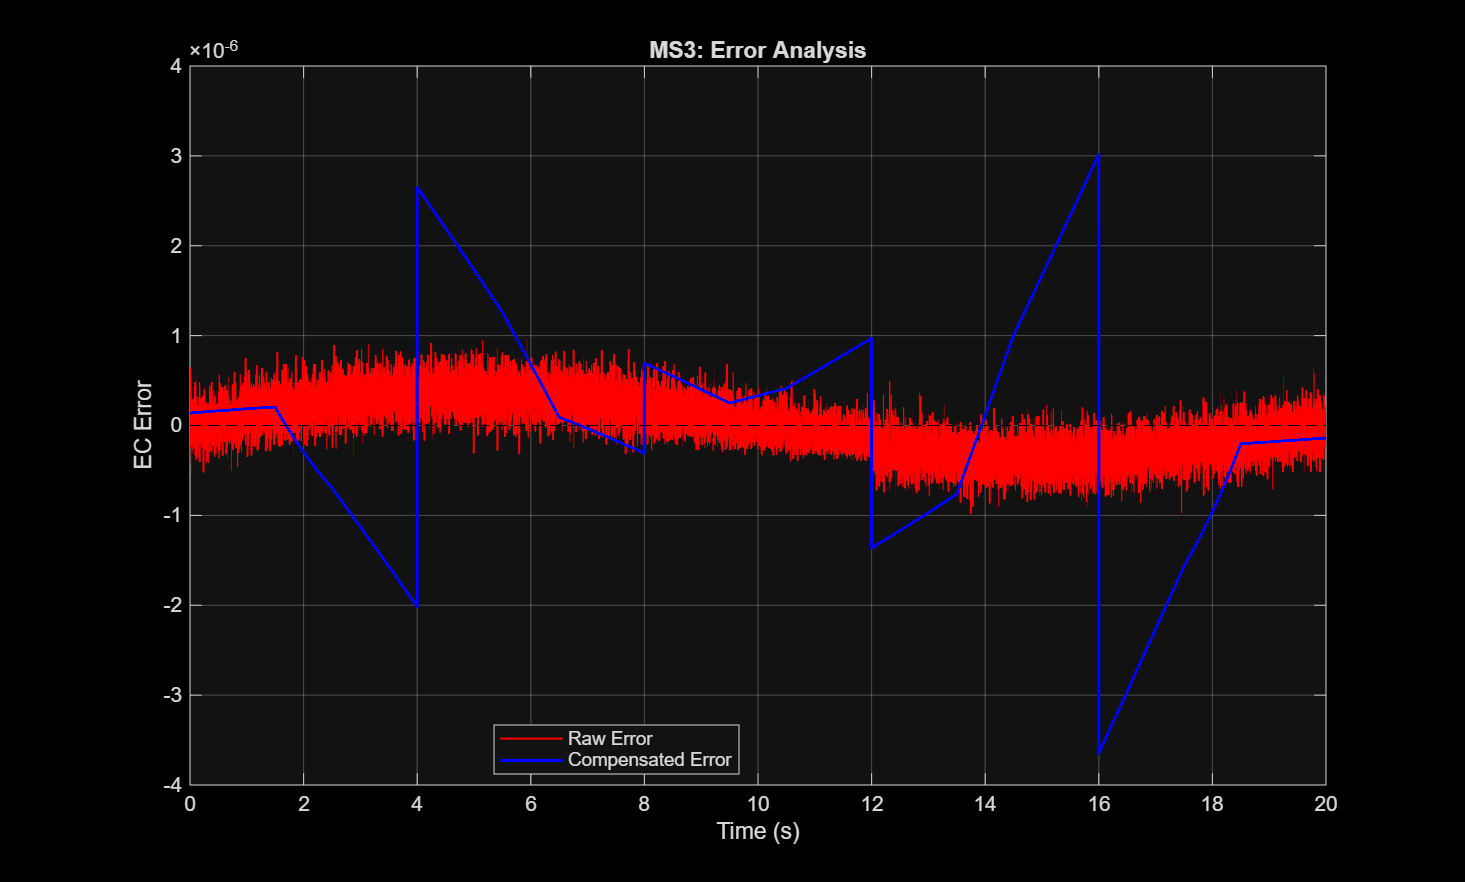
\includegraphics[width=\columnwidth]{page19_img1.jpeg}
\caption{EC estimation error: raw error (red) shows random noise fluctuations; compensated error (blue) exhibits large triangular peaks at step transitions due to filter over-smoothing.}
\label{fig:ms3_error}
\end{figure}

Fig.~\ref{fig:ms3_current} illustrates the current-domain signal processing chain. The compensated signal tracks the low-frequency envelope but lags behind abrupt steps, confirming the fundamental noise--bandwidth trade-off.

\begin{figure}[H]
\centering
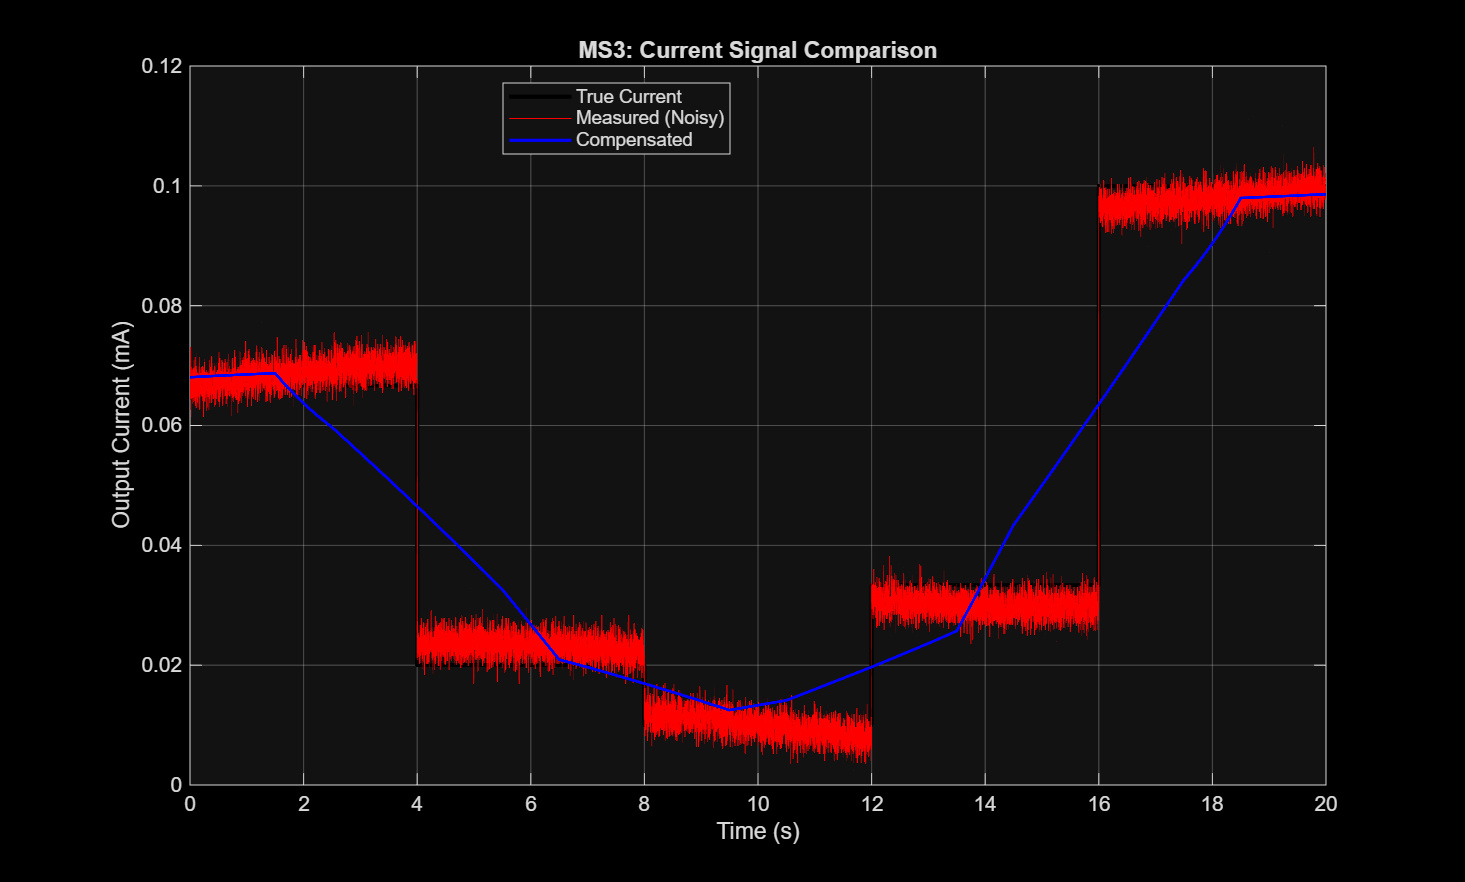
\includegraphics[width=\columnwidth]{page19_img2.jpeg}
\caption{Current signal comparison: true (black), measured with noise and drift (red), and compensated (blue). The filter smooths noise but cannot follow rapid EC transitions.}
\label{fig:ms3_current}
\end{figure}

Table~\ref{tab:ms3_metrics} quantifies the full-trajectory compensation performance. The raw measurement achieves 6.78\% RMSE ($10.17\%$ with the $N = 500$ stage alone), while the 5\,s window increases full-sequence RMSE to 27.25\% due to step over-smoothing---a result specific to the artificially fast 4\,s step trajectory. For slowly varying field soil EC (minutes to hours), active drift subtraction or adaptive filtering is still needed to remove slow baseline bias.

\begin{table}[H]
\centering
\caption{Full-Trajectory Noise Compensation Metrics (S/cm)}
\label{tab:ms3_metrics}
\begin{tabular}{lll}
\toprule
\textbf{Metric} & \textbf{Raw} & \textbf{Compensated} \\
\midrule
RMSE [S/cm] & $3.12 \times 10^{-7}$ & $1.25 \times 10^{-6}$ \\
RMSE (\% of mean EC) & 6.78\% & 27.25\% \\
Max Abs.\ Error [S/cm] & $9.77 \times 10^{-7}$ & $3.65 \times 10^{-6}$ \\
Mean Bias [S/cm] & $3.66 \times 10^{-9}$ & $-4.09 \times 10^{-9}$ \\
\bottomrule
\end{tabular}
\end{table}

\section{Commercial Sensor Evaluation}
\subsection{Application Requirements}
Quantitative requirements for agricultural soil EC monitoring are: conductivity range 5\,$\mu$S/cm to 200\,mS/cm, accuracy $<$5\% FS, response time $<$1\,s (90\% settling), and operating temperature 0--50$^\circ$C.

\subsection{Evaluated Sensors}
Three commercial sensors are compared against our optimized design:
\begin{enumerate}
\item \textbf{Atlas Scientific K\,1.0:} Professional-grade probe with 5--200{,}000\,$\mu$S/cm range, $\pm$2\% accuracy, and fringe-effect immunity~\cite{atlas2023}.
\item \textbf{Vernier CON-BTA:} Educational probe with automatic temperature compensation and three selectable ranges up to 20{,}000\,$\mu$S/cm~\cite{vernier2025}.
\item \textbf{METER 5TE:} Integrated probe measuring VWC, EC (0--23\,dS/m), and soil temperature with a 150\,ms response~\cite{meter2018}.
\end{enumerate}

\subsection{Datasheet Comparison}
Table~\ref{tab:datasheet} consolidates key specifications from manufacturer datasheets.

\begin{table}[H]
\centering
\caption{Commercial Sensor Specifications Comparison}
\label{tab:datasheet}
\resizebox{\columnwidth}{!}{%
\begin{tabular}{lllll}
\toprule
\textbf{Spec.} & \textbf{Atlas K\,1.0} & \textbf{Vernier} & \textbf{METER 5TE} & \textbf{Ours} \\
\midrule
Range [$\mu$S/cm] & 5--200k & 0--20k & 0--23k & 5--200k \\
Accuracy & $\pm$2\% & $\pm$2\% FS & $\pm$10\% & $\pm$5\% FS \\
Response (90\%) & 1\,s & 5\,s & 150\,ms & $<$100\,ms \\
Temp.\ Range & 1--110$^\circ$C & 0--80$^\circ$C & $-$40--60$^\circ$C & $-$10--60$^\circ$C \\
$K_{cell}$ [cm$^{-1}$] & 1.0 & 1.0 & N/A & 0.1 \\
Price & \$140 & \$150--200 & \$200--250 & Prototype \\
\bottomrule
\end{tabular}%
}
\end{table}

\subsection{Weighted Decision Matrix}
A weighted scoring matrix (Table~\ref{tab:decision}) evaluates each sensor across eight criteria. Weights are assigned based on application priority: accuracy (25\%), range (20\%), response time (15\%), temperature (10\%), environmental suitability (10\%), interference immunity (10\%), cost (5\%), and maintenance (5\%).

\begin{table}[H]
\centering
\caption{Weighted Decision Matrix (Scores 1--10)}
\label{tab:decision}
\resizebox{\columnwidth}{!}{%
\begin{tabular}{lccccc}
\toprule
\textbf{Criterion} & \textbf{Wt.\ (\%)} & \textbf{Atlas} & \textbf{Vernier} & \textbf{METER} & \textbf{Ours} \\
\midrule
Range Coverage & 20 & 10 & 6 & 7 & 10 \\
Accuracy & 25 & 10 & 9 & 6 & 8 \\
Response Time & 15 & 7 & 5 & 10 & 10 \\
Operating Temp. & 10 & 9 & 7 & 10 & 7 \\
Environ.\ Suit. & 10 & 8 & 6 & 10 & 9 \\
Interference Imm. & 10 & 9 & 8 & 7 & 8 \\
Cost & 5 & 8 & 7 & 5 & 10 \\
Maintenance & 5 & 9 & 8 & 9 & 7 \\
\midrule
\textbf{Total Score} & \textbf{100} & \textbf{9.00} & \textbf{7.05} & \textbf{7.80} & \textbf{8.75} \\
\bottomrule
\end{tabular}%
}
\end{table}

The Atlas Scientific K\,1.0 achieves the highest weighted score (9.00/10) due to its exceptional range, accuracy, and fringe-effect immunity. Our optimized $K_{cell} = 0.1$ design ranks second (8.75/10), demonstrating superior response time and sensitivity but requiring hardware validation.

\section{Discussion}
\subsection{Key Findings}
The Lagrangian-based RLC model accurately captures the sensor's second-order dynamics and enables systematic identification of performance bottlenecks. The critical insight is that the soil itself acts as the primary damper, causing the damping ratio to vary by nearly four orders of magnitude across the operating range. This variable damping fundamentally limits the sensor's ability to maintain uniform performance across soil types.

The geometric optimization ($K_{cell}: 1.0 \rightarrow 0.1\,\text{cm}^{-1}$) simultaneously addresses sensitivity and response speed through a single physical modification. The key trade-off is the distinction between the RC time constant ($\tau = 0.3$\,s) and the practical current settling time ($<$100\,ms): because the measured quantity is current rather than voltage, and the circuit is heavily overdamped, the resistive response dominates.

\subsection{Non-Linearity Perspective}
The sensor is inherently non-linear with respect to resistance ($I = V/R$) but linear with respect to conductivity ($I \propto \sigma$). The geometric optimization elevates fresh-water signals above the noise floor ($66.7\,\mu$A vs.\ $6.67\,\mu$A), enabling accurate readout of the linear $I$--$EC$ relationship and effectively bypassing the hyperbolic non-linearity issue.

\subsection{Signal Processing Trade-offs}
The noise compensation results highlight the fundamental conflict between noise suppression and transient tracking. The 5\,s filter window is optimal for slowly-varying real-world soil conditions but incompatible with the artificially fast test trajectory. Adaptive filtering or Kalman estimation would provide robust performance across diverse signal dynamics at the cost of increased computational complexity.

\subsection{Simulation vs.\ Commercial Reality}
The datasheet comparison validates key simulation assumptions: our predicted range matches the Atlas K\,1.0 exactly (5--200{,}000\,$\mu$S/cm), our $\pm$5\% accuracy target is conservative (commercial sensors achieve $\pm$2\%), and the sub-100\,ms response time is supported by the METER 5TE's 150\,ms specification. Temperature compensation remains a critical factor, as EC varies approximately 2\%/$^\circ$C~\cite{hayashi2004}. No commercial sensor uses $K_{cell} = 0.1\,\text{cm}^{-1}$, raising important questions about electrode fouling, fringe-effect sensitivity, and manufacturability that require hardware prototyping to resolve.

\section{Conclusion}
This paper presented the complete design cycle of a soil EC sensor for precision agriculture, from Lagrangian-based mathematical modeling through geometric optimization, signal processing, and commercial benchmarking. The baseline RLC model ($L_{coil} = 3\,\mu$H, $C_{dl} = 10\,\mu$F, $K_{cell} = 1.0\,\text{cm}^{-1}$) revealed critical limitations: 76.8\% FSO non-linearity, $6.67\,\mu$A fresh-water sensitivity, and 6\,s settling time. Geometric optimization to $K_{cell} = 0.1\,\text{cm}^{-1}$ achieved a 10$\times$ sensitivity gain and $>$60$\times$ faster settling while maintaining $>$2\,MHz bandwidth. A dual-window moving average filter effectively suppressed 30\,dB noise but demonstrated the inherent trade-off between noise rejection and transient tracking speed. The weighted decision matrix identified the Atlas Scientific K\,1.0 (score: 9.00/10) as the best commercial solution, while our optimized design (8.75/10) offers compelling advantages in fresh-water sensitivity and response speed that warrant 6--12 months of field validation. Future work should focus on hardware prototyping, adaptive filtering algorithms, and temperature compensation to bridge the gap between simulation and practical deployment.

\begin{thebibliography}{9}
\bibitem{atlas2023}
Atlas Scientific, ``Conductivity Probe K 1.0 Datasheet,'' 2023. [Online]. Available: \url{https://atlas-scientific.com/probes/conductivity-probe-k-1-0/}

\bibitem{vernier2025}
{\raggedright
Vernier Software \& Technology, ``Conductivity Probe User Manual (CON-BTA),'' 2025. [Online]. Available: \url{https://www.vernier.com/manuals/con-bta/}\par}

\bibitem{meter2018}
METER Group, Inc., ``5TE Water Content, EC and Temperature Sensors Manual,'' 2018. [Online]. Available: \url{https://www.misure.net/sites/default/files/pdf/20435_5TE_Manual_Web.pdf}

\bibitem{rhoades1999}
J.~D.~Rhoades, F.~Chanduvi, and S.~Lesch, ``Soil Salinity Assessment: Methods and Interpretation of Electrical Conductivity Measurements,'' FAO Irrigation and Drainage Paper 57, Rome, Italy, 1999.

\bibitem{ayers1985}
R.~S.~Ayers and D.~W.~Westcot, ``Water Quality for Agriculture,'' FAO Irrigation and Drainage Paper 29, Rev.\ 1, Rome, Italy, 1985.

\bibitem{corwin2005}
D.~L.~Corwin and S.~M.~Lesch, ``Apparent soil electrical conductivity measurements in agriculture,'' \emph{Computers and Electronics in Agriculture}, vol.~46, no.~1--3, pp.~11--43, 2005.

\bibitem{fraden2016}
J.~Fraden, \emph{Handbook of Modern Sensors: Physics, Designs, and Applications}, 5th~ed.\hspace{0.5em} Cham, Switzerland: Springer, 2016.

\bibitem{ogata2010}
K.~Ogata, \emph{Modern Control Engineering}, 5th~ed.\hspace{0.5em} Upper Saddle River, NJ, USA: Prentice Hall, 2010.

\bibitem{hayashi2004}
M.~Hayashi, ``Temperature-electrical conductivity relation of water for environmental monitoring and geophysical data inversion,'' \emph{Environmental Monitoring and Assessment}, vol.~96, no.~1--3, pp.~119--128, 2004.

\end{thebibliography}

\end{document}
